\documentclass[12pt,a4paper]{article}

\usepackage[T1]{fontenc}
\usepackage[utf8]{inputenc}
\usepackage{lmodern}
\usepackage[english]{babel}
\usepackage[margin=2.5cm]{geometry}
\usepackage{xcolor}
\usepackage{listings}
\usepackage{enumitem}
\usepackage{titlesec}
\usepackage{needspace}
\usepackage{graphicx}
\usepackage[hidelinks]{hyperref}

\titleformat{\section}{\Large\bfseries}{\thesection.}{0.5em}{}
\titleformat{\subsection}{\large\bfseries}{\thesubsection.}{0.5em}{}

\definecolor{codebg}{gray}{0.96}
\lstset{
    basicstyle=\ttfamily\small,
    backgroundcolor=\color{codebg},
    frame=single,
    rulecolor=\color{gray!40},
    breaklines=true,
    columns=fullflexible,
    keepspaces=true,
    showstringspaces=false,
    upquote=true,
    aboveskip=8pt,
    belowskip=8pt
}

\setlist[enumerate]{itemsep=6pt}
\setlength{\emergencystretch}{3em}

\begin{document}

\begin{titlepage}
    \centering
    Ministerul Educa\c{t}iei \c{s}i Cercet\u{a}rii al Republicii Moldova\\[0.4cm]
    \textbf{Universitatea Tehnic\u{a} a Moldovei}\\[0.4cm]
    Facultatea Calculatoare, Informatic\u{a} \c{s}i Microelectronic\u{a}\\[0.2cm]
    Program: Software Engineering

    \vspace{3cm}

    {\LARGE \textbf{Operating Systems}}

    \vspace{1.2cm}

    {\Large \textbf{Laboratory Work No. 9}}\\[0.6cm]
    {\LARGE \textbf{Watching System Calls with strace}}\\[0.3cm]
    Track A: The Real OS, from the Outside (Linux)

    \vspace{3cm}

    \begin{flushright}
        \textbf{Elaborated by:}\\
        st. gr. FAF-243\\
        Veacheslav Morari\\[0.6cm]
        \textbf{Verified by:}\\
        Patricia Re\c{t}man
    \end{flushright}

    \vfill
    Chi\c{s}in\u{a}u -- 2026
\end{titlepage}

\tableofcontents
\newpage

\section*{Introduction}
\addcontentsline{toc}{section}{Introduction}

In the lecture we crossed the door between a program and the kernel: the system call. The purpose of this laboratory work is to \emph{watch} that door from the outside. The tool \texttt{strace} prints every system call a program makes. In the three parts of the lab we first look at the calls of a familiar command, then write a tiny C program that uses \texttt{open}, \texttt{write} and \texttt{read} directly, and finally count the kinds of system calls a program makes during one run. The work was done on Ubuntu 26.04 with \texttt{strace} from the \texttt{apt} repository.

\section{See the calls of a real command}

The first part looks at the calls that \texttt{ls -l} makes while listing the current directory. \texttt{strace} with the flag \texttt{-e trace=openat,read,write,close} limits the output to those four calls, which are enough to understand the pattern:

\begin{lstlisting}
$ strace -f -e trace=openat,read,write,close ls -l | head -40
\end{lstlisting}

The output showed a burst of \texttt{openat}/\texttt{read}/\texttt{close} while \texttt{ls} loads its shared libraries (\texttt{libc.so.6}, \texttt{libselinux.so.1}, \texttt{libpcre2-8.so.0}), then opens \texttt{/proc/filesystems} and \texttt{/proc/self/maps}, reads coreutils locale files, and finally opens the directory \texttt{"."} itself. The listing is produced by a single \texttt{write}:

\begin{lstlisting}
openat(AT_FDCWD, ".", O_RDONLY|O_NONBLOCK|O_CLOEXEC|O_DIRECTORY) = 3
close(3)
write(1, "total 0\n", 8)
\end{lstlisting}

\subsection{Observations}

\texttt{ls} prints to the screen with the \texttt{write} system call, on file descriptor \textbf{1}, the standard output. Even a small command like \texttt{ls -l} on an empty directory makes dozens of system calls: most of them are the dynamic loader fetching shared libraries, and only a few are the real work (opening the directory and writing the listing). This is a first glimpse of how much the kernel does for a single command.

\section{A program that calls the kernel directly}

The second part uses a small C program, \texttt{syscalls.c}, that reaches for the kernel without any library wrapper around the three main calls. It creates a file, writes a short message, closes it, opens it again, reads the message back and closes it. The complete source is in \texttt{syscalls.c}.

\begin{lstlisting}[language=C]
int fd = open("note.txt", O_CREAT | O_WRONLY | O_TRUNC, 0644);
printf("open returned descriptor %d\n", fd);
ssize_t n = write(fd, msg, strlen(msg));
printf("write sent %zd bytes\n", n);
close(fd);

fd = open("note.txt", O_RDONLY);
char buf[64];
n = read(fd, buf, sizeof(buf) - 1);
buf[n] = '\0';
printf("read got %zd bytes: %s", n, buf);
close(fd);
\end{lstlisting}

Compiled with \texttt{gcc -Wall -Wextra -o syscalls syscalls.c} and run, the program produced the expected three lines:

\begin{lstlisting}
open returned descriptor 3
write sent 14 bytes
read got 14 bytes: hello, kernel
\end{lstlisting}

The same run under \texttt{strace -e trace=openat,write,read,close ./syscalls} showed the calls hidden behind the C code. Figure \ref{fig:strace} shows the output.

\begin{figure}[h]
    \centering
    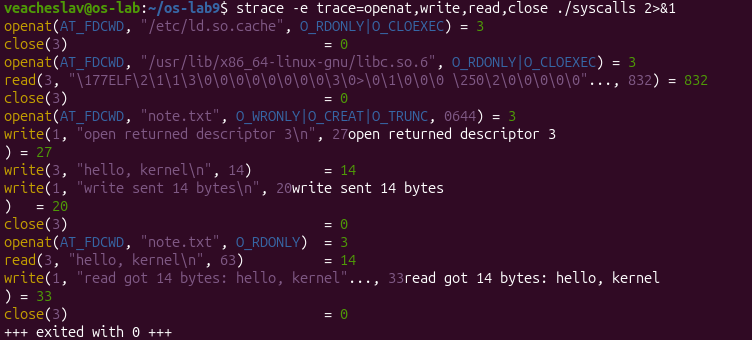
\includegraphics[width=0.85\textwidth]{screenshots/fig1.1_strace_syscalls.png}
    \caption{\texttt{strace} output for \texttt{syscalls}. The three calls we wrote (\texttt{openat}, \texttt{write}, \texttt{read}, \texttt{close}) appear after the loader has opened \texttt{libc.so.6}. The descriptor returned by every \texttt{openat} is 3.}
    \label{fig:strace}
\end{figure}

\subsection{Observations}

The descriptor returned by the first \texttt{openat} on \texttt{note.txt} is \textbf{3}, not 0, 1 or 2, because every new process is born with three open file descriptors already in place: 0 is the standard input (the keyboard, inherited from the shell), 1 is the standard output (the terminal), and 2 is the standard error (also the terminal). The kernel always gives a new open the smallest free number, and the first free number after 0, 1 and 2 is 3.

Figure \ref{fig:strace} also shows the printf output interleaved with the strace lines. Each \texttt{printf} eventually becomes a \texttt{write(1, "\dots", n)} to standard output, which is why those lines appear under strace too. The library opens \texttt{libc.so.6} once at startup, which uses a few descriptor 3 slots that are closed immediately after reading the ELF header.

\section{Count one kind of call}

The third part measures how many calls of each kind a single run of the program makes. \texttt{strace -c} prints a summary table instead of the live output:

\begin{lstlisting}
$ strace -c ./syscalls
\end{lstlisting}

The result for one run of \texttt{./syscalls} is shown in Figure \ref{fig:strace-c}.

\begin{figure}[h]
    \centering
    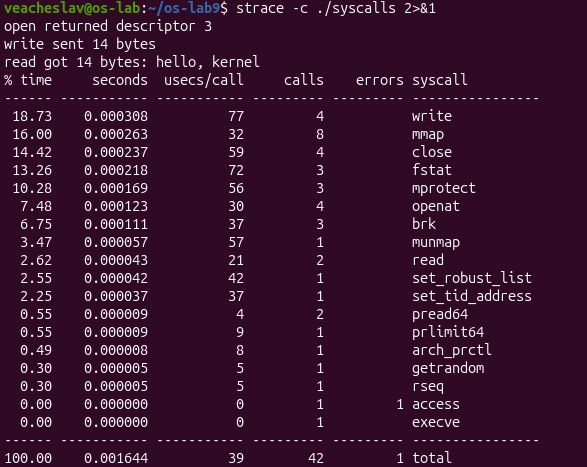
\includegraphics[width=0.85\textwidth]{screenshots/fig2.1_strace_count.png}
    \caption{\texttt{strace -c ./syscalls}: 42 system calls in total, grouped by kind. The counts (not the \% time, which varies between runs) are deterministic for this program.}
    \label{fig:strace-c}
\end{figure}

\subsection{Observations}

The program makes \textbf{42 system calls in total}, far more than the three I wrote by hand. Most of them belong to the setup phase: 8 \texttt{mmap} calls and 3 \texttt{brk} calls grow the address space and map libc into memory; 3 \texttt{mprotect} calls set the right permissions on those regions; 3 \texttt{fstat} calls look at libc. Among my calls, \texttt{openat} appears 4 times (the loader's two opens of \texttt{/etc/ld.so.cache} and \texttt{libc.so.6}, plus my two opens of \texttt{note.txt}), \texttt{close} appears 4 times for the same reason, \texttt{read} appears twice (one for libc, one for \texttt{note.txt}), and \texttt{write} appears 4 times (one for the data in \texttt{note.txt} and three \texttt{write}s produced by the three \texttt{printf} calls).

The \texttt{-c} flag of \texttt{strace} is useful when the question is \emph{how many} of a given call a program makes rather than \emph{what order}. Running the same command twice gives the same counts but slightly different timings, as Figure \ref{fig:strace-c} confirms when compared with earlier runs.

\section*{Conclusion}
\addcontentsline{toc}{section}{Conclusion}

Watching a program from the outside with \texttt{strace} turns the system call from an abstract idea into a concrete event: every line of the output is a visible crossing of the user--kernel boundary. The experiments showed that even a short program spends most of its calls on setup (loader, memory mapping) and only a few on real work, that file descriptors are small integers allocated by the kernel in the smallest-free-number order (which is why the first \texttt{open} returned 3), and that counting calls with \texttt{strace -c} is a quick way to compare the behaviour of programs. The same idea --- print every system call a process makes --- will be built from scratch in Lab 10, where \texttt{strace} is replaced by a new system call added to xv6.

\end{document}
